\documentclass[preprint,11pt]{aastex}

% Copyright 2012, 2013 The GalSim developers:
% https://github.com/GalSim-developers
%
% This file is part of GalSim: The modular galaxy image simulation toolkit.
%
% GalSim is free software: you can redistribute it and/or modify
% it under the terms of the GNU General Public License as published by
% the Free Software Foundation, either version 3 of the License, or
% (at your option) any later version.
%
% GalSim is distributed in the hope that it will be useful,
% but WITHOUT ANY WARRANTY; without even the implied warranty of
% MERCHANTABILITY or FITNESS FOR A PARTICULAR PURPOSE.  See the
% GNU General Public License for more details.
%
% You should have received a copy of the GNU General Public License
% along with GalSim.  If not, see <http://www.gnu.org/licenses/>
%

% packages for figures
\usepackage{graphicx,times}
% packages for symbols
\usepackage{latexsym,amssymb,hyperref}
% AMS-LaTeX package for e.g. subequations
\usepackage{amsmath}

%=====================================================================
% FRONT MATTER
%=====================================================================

\slugcomment{\today}

%=====================================================================
% BEGIN DOCUMENT
%=====================================================================

\begin{document}

\setlength{\parskip}{2.0ex plus 0.5ex minus 0.5ex}
\setlength{\parindent}{0cm} 

\title{Why Have We Updated the Metrics for GREAT3?}

You may have noticed that your metric scores in the GREAT3
Leaderboards have changed slightly.  These changes will be most
noticeable for the highest scoring entries, but \emph{all} scores have
changed by some amount.  This document will explain why these change
were made, and give the definitions of the new metrics.

\section{Background}\label{sec:bg}
As mentioned in the first versions of the GREAT3 Handbook (Mandelbaum
et al 2013), we always felt it
might be necessary to update the metrics as we received more
information about methods in the form of entries to GREAT3.  In
particular we felt it might be necessary to \emph{renormalize} the
metrics, to make it so that a method scores $\sim 1000$ if it reaches
target performance.

So why would either the constant shear metric ($Q_{\rm c}$) or
variable shear metric ($Q_{\rm v}$) need renormalization?

To answer this question, let us consider a simple model of the
contributions to an observation of a (complex) gravitational shear $g_{\rm obs}$.
We may write this as a combination of the gravitational reduced shear $g$, galaxy intrinsic ellipticity
$g_{\rm int}$, and a measurement noise term $g_{\rm noise}$ due to the
pixel noise in galaxy images:
\begin{equation}
g_{\rm obs} \simeq g + g_{\rm int} + g_{\rm noise}.
\end{equation}
As they are both noise terms as far as shear measurement is concerned,
it is not uncommon in weak lensing to refer to $g_{\rm int}$ as \emph{shape
  noise} and $g_{\rm noise}$ as \emph{measurement noise} (perhaps this sounds
better than `noise noise'...).

In GREAT3 we have designed our experiments with inherent symmetries
that allow us to cancel out the contributions from intrinsic ellipticity
$g_{\rm int}$ to uncertainty on shear (see Mandelbaum et al 2013).
This allows us to reduce the  total data volume of the challenge
significantly.  However, we have not devised a means to cancel out
contributions from $g_{\rm noise}$, and it is this noise which
ultimately sets data volume required to reach a given sensitivity on
shear biases in methods.

When simulating the performance of various metrics -- for many different
$Q_{\rm c}$ and $Q_{\rm v}$ have been tested using simulated GREAT3
submissions with a range of biases -- we modelled the measurement
noise as Normally distributed with zero mean and standard deviation
set by the variable \texttt{NOISE\_SIGMA}:
\begin{equation}
g_{\rm noise} \sim \mathcal{N}(0, \texttt{NOISE\_SIGMA}^2).
\end{equation}
For all the simulations that went into testing and normalizing the
metrics in the GREAT3 Handbook, a value of \texttt{NOISE\_SIGMA} =
0.05 was estimated as being appropriate to our images.

This figure was based on the decision to include only galaxy images
with signal-to-noise ratio (SNR) $\gtrsim 20$ in GREAT3, using the SNR
defined by Bridle et al (2008).  Assuming a steep distribution of
galaxy SNRs so that the population is dominated by objects with ${\rm
  SNR} \sim 20$, and invoking the approximate, experimentally
supported `rule of thumb' $g_{\rm noise} \sim ({\rm SNR})^{-1}$, gave
rise to the estimate $\texttt{NOISE\_SIGMA} \simeq 0.05$ used in the
simulations of metrics and the calculation of an appropriate
normalization factor for $Q_{\rm v}$.

\section{Galaxy image signal-to-noise}\label{sec:snr}
What we have realised about the GREAT3 galaxy images is that the SNR
definition itself has a significant impact on the SNR value assigned
to each image.

The Bridle et al (2008) definition uses prior knowledge of the
convolved galaxy light profile and in that respect is an optimal
(matched filter) estimate of the SNR.  It also means that it cannot be
used as an estimate of SNR in real data, where this light profile is
unknown.

A definition of SNR often used in practice comes from an estimate of
the flux within a given aperture, divided by an estimate of the
uncertainty on the flux in the same aperture.  Using the
\textsc{SExtractor} software (Bertin \& Arnouts 1996) we can define a
practical of SNR as $\texttt{FLUX\_AUTO} / \texttt{FLUXERR\_AUTO}$.
Using this definition, and \textsc{SExtractor} detection settings that
securely locate all objects, we find that 99\% of objects in the
ground (space) data have SNR~$>$~9.97~(11.7), and 90\% have
SNR~$>$~13.5 (14.4 for space).  In Figure \ref{eq:snr} we plot a
typical distribution of these SNR values for objects in one of the
GREAT3 galaxy image files.  A large fraction of these objects give an
estimated SNR~$<$~20 using the  $\texttt{FLUX\_AUTO} /
\texttt{FLUXERR\_AUTO}$ definition.

\begin{figure}\label{eq:snr}
\begin{center}
%\epsscale{num}
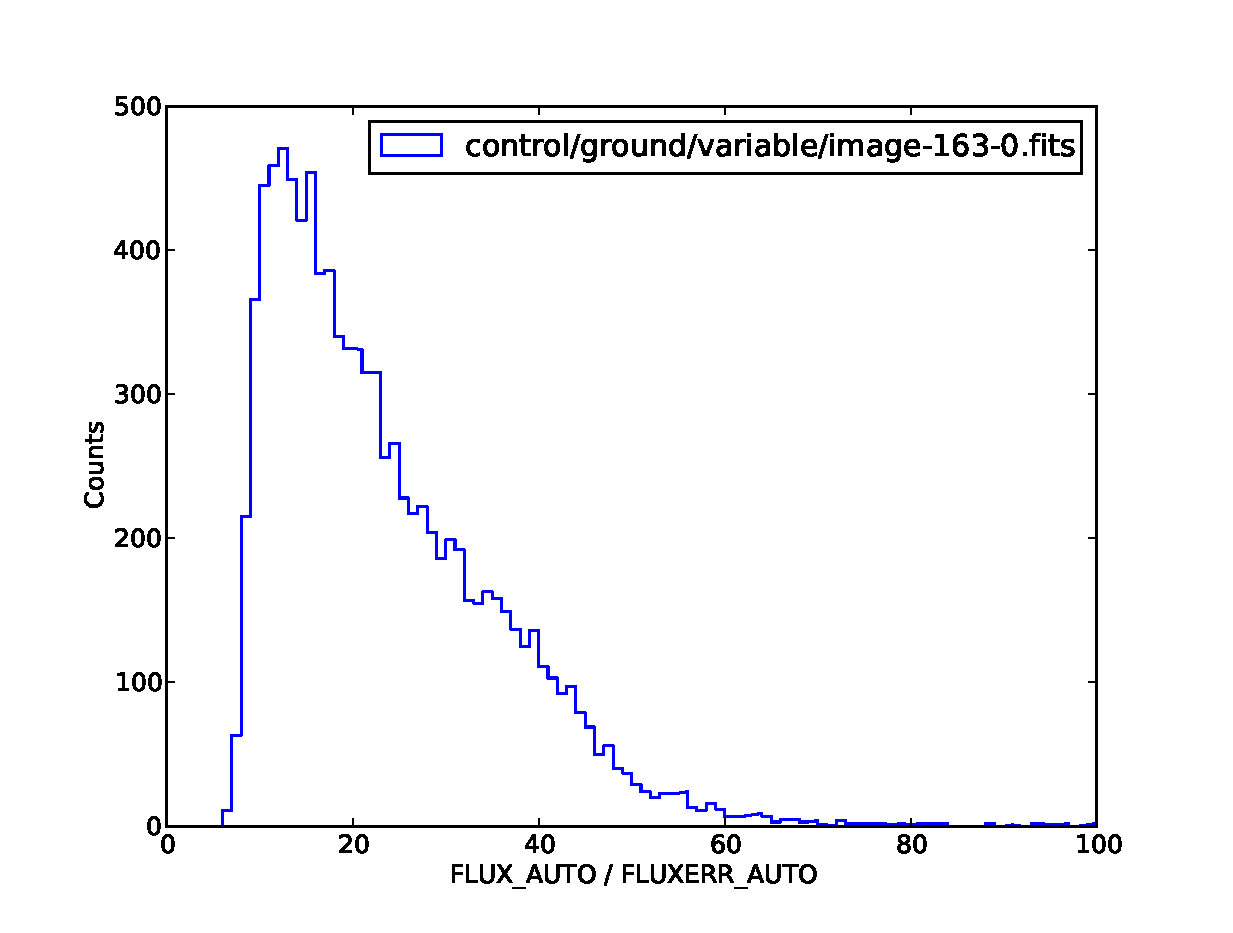
\includegraphics[width=\textwidth]{snr_cvg.eps}
\caption{Distribution of $\texttt{FLUX\_AUTO} /
  \texttt{FLUXERR\_AUTO}$ for galaxy postage stamps in
  \texttt{image-163-0.fits} in the control/ground/variable branch of GREAT3.}
\end{center}
\end{figure}

\section{New Estimates for \texttt{NOISE\_SIGMA}}\label{sec:ns}
Because the typical SNR of galaxy images in GREAT3 is lower than
envisaged using a practical definition of SNR, the scaling
relationship used to estimate $\texttt{NOISE\_SIGMA}$ has been found
to be wrong.   Based on results coming in from early submissions, and
internal validations of GREAT3, we have found that better estimates of
the typical standard deviation of measurement noise are in fact:
\begin{itemize}
\item[] $\texttt{NOISE\_SIGMA} \simeq 0.15$ for the branches simulating
  observations from the ground;
\item[] $\texttt{NOISE\_SIGMA} \simeq 0.10$ for the branches simulating
  observations from space.
\end{itemize}
The excess measurement noise for the ground branch data comes from the
additional uncertainty on galaxy shape due to the larger convolving
Point Spread Function (PSF) in these simulations.  This is a factor
that is not included in the approximate rule of thumb we described in
Section~\ref{sec:bg}: it is of relevance due to the realistically
large PSF-to-galaxy size ratio in the simulations of the ground
observations, based on galaxy models from HST images as described in
Mandelbaum et al (2013).

\section{The Constant Shear Metric $Q_{\rm c}$}\label{sec:qc}
The increased measurement noise variance leads to greater
uncertainty in the values of $m_i$ and $c_i$ used in the determination
of $Q_{\rm c}$.  This was not something that was significant in
simulations that used \texttt{NOISE\_SIGMA} = 0.05, but with the
improved estimates described in Section \ref{sec:ns} this is no longer
the case.

To counter this effect, we have modified the $Q_{\rm c}$ metric. We
now add the $m$ and $c$ values in quadrature with a noise term
$\sigma_\text{min}^2$ that is designed to ensure that the scores for
methods with very low-$m$ and $c$ are not dominated by noise, which
can give spurious fluctuations to very high $Q_{\rm c}$ for methods
without significant bias.  The constant shear branch metric is then
defined as
\begin{equation}\label{eq:q_c}
Q_{\rm c} = \frac{2000}{\sqrt{ \sigma_\text{min}^2 + \displaystyle\sum_{i=1,2} \left(
      \frac{m_i}{m_{\rm target}} \right)^2 + \left( \frac{c_i}{c_{\rm target}} \right)^2 }};
\end{equation}
see Mandelbaum et al (2013).  Based on simulations, we adopt a value of
$\sigma_\text{min}^2$ = 4 (1) for ground (space) branches.  These
correspond roughly to the intrinsic uncertainties in the quadrature
sum of $m_i / m_{\rm target}$ and $c_i / c_{\rm target}$ due to
measurement noise. For methods with $m_i$ or $c_i$ noticably above the
targets, the $\sigma^2_{\rm min}$ term is essentially irrelevant.

\section{The Variable Shear Metric $Q_{\rm v}$}\label{sec:qv}


\end{document}
